\chapter{Algorithmics}
\label{chap:algorithmics}

\chapterquote{I'm smart enough to know that I'm dumb. }{Richard Feynman}

\chapterquote{Beware of bugs in the above code; I have only\\ proved it correct, not tried it.}{Donald  Knuth}

This final technical chapter will discuss some of the algorithmic foundations and consequences of the graph-simplex correspondence. Vis-\`{a}-vis foundations, we will chiefly be concerned with transitioning between a graph and its various simplices. We will explore lower bounds for how quickly this can be done if we wish to obtain the precise result\footnote{Ignoring issues of floating point number accuracy.}, and whether we can ``approximate'' any of the constructions (e.g., given the graph $G$ can we quickly obtain a simplex which serves as an approximation\footnote{The notion of approximating a simplex is rather ambiguous and will be expounded upon at a later time.} to $\splx_G$.) With respect to algorithmic consequences, we will attempt to leverage knowledge we have in the hitherto mostly unrelated areas of computational graph theory and high-dimensional computational geometry to draw new conclusions about the complexity of several problems. For instance, if a  graph theoretic problem has an analogue in the simplex, any fact regarding the problem's difficulty---whether it's \NP-complete, say---translates to an immediate result concerning its geometric counterpart. In particular, since the simplex of a graph can be generated in polynomial time given the graph (due to the fact that an eigendecomposition can be computed in polynomial time) and vice versa, problems which are solvable in polynomial time in either the simplex or graph domain  translate to polynomially solvable (yet perhaps not optimal!) problems in the other domain. Likewise, problems which are \NP-hard in one domain have analogues which are \NP-hard in the other. 

For the benefit of the reader unfamiliar with computational complexity and reductions, we begin the chapter with a short section containing this background material. We will also discuss computational representations of a simplex therein. 

\section{Preliminaries}
\label{sec:algorithmics_prelims}
\paragraph{Asymptotics.}
Asymptotic notation will be used to analyze the running time of various algorithms. We use the standard definitions---see any reference text on algorithm design for more background (e.g., \cite{kleinberg2006algorithm}). Let $f,g:U\subset \R \to \R$ be functions. Write $f=O(g)$ (or $f(n)=O(g(n))$) if $\limsup_{x\to \infty}|f(x)/g(x)|<\infty$, and $f=\Omega(g)$ if $g=O(f)$. Write $f=o(g)$ as $x\to c$ if $\lim_{x\to \infty}|f(x)/g(x)|=0$ and $f=\omega(g)$ if $g=o(f)$. If $f=O(g)$ and $f=\Omega(g)$ we write $f=\Theta(g)$. We will also use the tilde to hide polylog factors. Say $f=\tO(g)$ if $f(n) = O(g(n) \log^c n)$ and $f=\tOmega(g)$ if $f(n) = \Omega(g(n) \log^{-c}n)$, for some $c\geq 0$. 


\paragraph{Simplex representations.}
In order to discuss the algorithmics pertaining to simplices and convex polyhedra in general, we must discuss how such objects are represented by a machine. Clearly, we cannot simply enumerate all the points enclosed by a body in high-dimensional space. Instead we must concisely represent the boundaries of the polytope. The two most common such descriptions are 
\begin{itemize}
	\item \textsf{V}-\emph{description}, in which we are given the vertex vectors of the polytope; 
	\item \textsf{H}-\emph{description}, in which we are given the parameters of the half-spaces whose intersection defines the polytope. That is, if $\ssplx=\bigcap_i \{\x:\la \z_i,\x\ra \geq b_i\}$, then an \hdesc of $\ssplx$ would be the vectors $\{\z_i\}$ and the scalars $\{b_i\}$. 
\end{itemize}

It's not at all clear whether these descriptions are equivalent in the sense that one can easily generate one from the other. Indeed, the complexity of vertex enumeration (generating a \vdesc from an \hdesc) and facet enumeration (generating an \hdesc from a \vdesc) remains an open problem for general polytopes~\cite{kaibel2003some}, although there exist polynomial time algorithms when the polytopes are simplices (e.g., \cite{bremner1998primal}). We will return to this fact later on. 

We end by remarking that when discussing general  polytopes, we continue  to work  in $\R^{n-1}$ as a vector space. Thus,  the vertices of the polytope are still vectors which begin at the origin. 

\paragraph{Reductions.}
Some background on computational models and reductions will also be useful. For more details see~\cite{kleinberg2006algorithm} or \cite{knuth2011art}. We will use the typical computational model for analyzing algorithms. Without diving too far into the minutiae, we assume that single arithmetic operations require $O(1)$-time, i.e., constant. We will analyze the runtime of an algorithm as a function of how many bits it takes to represent the input. A common tool for providing upper bounds on the runtime of an algorithm is to ``reduce'' it to a problem for which a bound is already known. Assume problem $P$ requires time $\Omega(f_P(n))$ to solve---meaning that \emph{any} algorithm requires time $\Omega(f_P(n))$---where $n$ represents the size of the input and $f_P(n)$  is some function of $n$, e.g., $f_P(n) =  n^2\log n$. Let $Q$ be a distinct problem and suppose that for every instance of $P$ we can transform the input of $P$ to a valid input for $Q$, and transform the output of $Q$ to a valid output of $P$, both in time $O(f_P(n))$.  We have then established that $f_Q(n) = \Omega(f_P(n))$, where $f_Q$ is the runtime required to solve $Q$, since we can solve $P$ in time $f_Q(n) + O(f_P(n))$ by transforming any input to $P$ to the input of $Q$, solving $Q$, and transforming the output back. 
In  this case we say that $P$ \emph{has been reduced to  $Q$},  or that \emph{$Q$ was reduced from $P$}.
Such a technique will be used extensively throughout the next few sections. 

\paragraph{The complexity classes \NP, \NP-hard, and \NP-Complete.}
For brevity, we restrict ourselves to a very brief presentation of these concepts. The interested reader can find more background in any reference  on computational  complexity theory. 

The class \NP  is  the set of all decision problems\footnote{That is,  problems  to which we seek a yes/no answer.} which have solutions which are \emph{verifiable} in polynomial time. It is possible, for example, to check  in polynomial time whether  a given  set is in fact an independent set of a certain size. Thus the decision variant of \iset lies in \NP. \NP stands for ``non-deterministic polynomial time'', as it is formally the set of all  decision problems solvable by a non-deterministic Turing  machine in polynomial time~\cite{papadimitriou2003computational}. 

The class \NP-hard comprises all the problems to  which  any problem in \NP can be reduced in polynomial time (see above). That is, $P\in\NP$-hard iff for all  $Q\in\NP$,  $Q$ can be  reduced to $P$ in polynomial time. Thus,  to show that $P\in\NP$-hard, it suffices to reduce another problem $R\in\NP$-hard to  $P$ (in polynomial time) since,  in this  case, if all problems in \NP are  reducible  to  $R$  they are in turn  reducible  to  $P$. We  tend to think of \NP as the set of ``hard'' problems. 

Finally,  the class \NP-complete is the intersection of the classes \NP and  \NP-hard. Informally then, it is  the  class of all ``hard'' decision problems. 

\begin{figure}
	\centering
	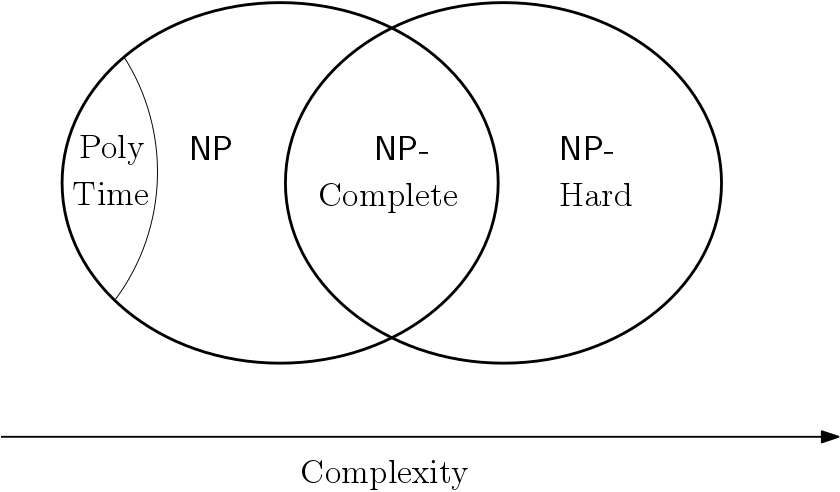
\includegraphics[scale=0.28]{NP_diagram}
	\caption{Illustration of the relationships between the  classes \NP,  \NP-hard, and \NP-complete. ``Poly-time'' refers to problems with polynomial time solutions. Such algorithms can trivially be verified  in polynomial time, hence  are a  subset of problems in \NP. We emphasize that the diagram is  for intuitive purposes only,  and may not reflect the true relationships between these classes. For example, in  the unlikely  case that \textsf{P}=\NP (i.e., all problems in  \NP are solvable in polynomail time), then the regions ``Poly time'', \NP and \NP-complete coincide. Additionally, the relative sizes of the regions above say  nothing about  their  true  cardinalities.}
\end{figure}



\section{Computational Complexity}
\label{sec:algorithmics_complexity}

In this section we investigate the relationships between problems in one domain---either the graph-theoretic or geometric domain---and their analogues in the other. The following result exemplifies the power of the graph-simplex correspondence in yielding results which seem otherwise difficult to obtain (certainly more difficult than the following proof, at any rate).  
It was first stated by Devriendt and Van Mieghem~\cite{devriendt2018simplex} for inverse combinatorial  simplices, and can be slightly generalized as follows.  

\begin{lemma}
	\label{lem:altitude_hard}
	Computing the altitude of minimum length in any simplex is \NP-hard. 
\end{lemma}
\begin{proof}
	The relationship $\norm{\alt(\splx^+_U)}_2^2 = w(\partial U)^{-1}$ (Lemma \ref{lem:alt}) for the inverse simplex of a graph $G$ demonstrates that the problem of computing a minimum length altitude in any hyperacute simplex is \NP-hard, because computing the  maximum weight cut in any weighted graph is \NP-hard~\cite{karp1972reducibility}.  Since the  class  of all hyperacute simplices is contained in the class of all simplices, the result follows.  (We note that formally, we have reduced the maximum  cute problem to the minimum altitude problem.) 
\end{proof}

\begin{remark} In  the above statement and its proof, the description of the polytope and simplex was not specified. This is due to the fact that---as discussed above---for simplices there is a polynomial time algorithm to translate between the various descriptions. With regard to \NP-completeness therefore, the description makes no difference. Consequently, we will continue to ignore this distinction for the remainder of this section. 
\end{remark}


\begin{remark}
Altitudes do  not have  an analogue in general polyhedra. However, for  those problems which do have analogues, 
if they are \NP-hard in hyperacute simplices then are so in general polyhedra (since simplices are a subclass of polyhedra). Henceforth, we might use this observation  without justification. 
\end{remark}


The remainder of this section is dedicated to obtaining more results of this type. 

We begin by investigating independent sets. Given a graph $G=(V,E,w)$, recall that an \emph{independent set} is a subset $I\subset V$ such that if $i,j\in I$ then $(i,j)\notin E$. 
The weight of an independent set is nicely described by the Laplacian quadratic form. If $I$ is an independent set note that $\partial(i)\cap I^c=\partial(i)$ for all $i\in  I$; otherwise $I$ would contain two vertices  which share an edge.
Therefore, 
\begin{align*}
w(\delta I) = \sum_{i\in  I}\sum_{j\in I^c} w(i,j) = \sum_{i\in I}\sum_{j\in \partial(i)\cap I^c} w(i,j) = \sum_{i\in  I}\sum_{j\in  \partial(i)}w(i,j) = \vol(I),
\end{align*}
so
\begin{align*}
    \Lf(\bchi_I) = \sum_{i\sim j}w(i,j)(\bchi_I(i)-\bchi_I(j))^2 = \sum_{i\in I}\sum_{j:j\sim i} w(i,j) = \vol(I)=w(\partial I),
\end{align*}
where the second inequality again follows from the fact that $I$ is an independent set. 

The \iset problem involves finding the largest independent set in a given  graph or,  in  the decision variant,  whether there exists an independent  set of size at least  $k$ for a given $k$.  
Suppose we assign each vertex $i$ a weight $f(i)\geq 0$. The \mwis problem consists of maximizing $f(I)\equiv \sum_{i\in I}f(i)$ over all independent sets $I$. Clearly \mwis is \NP-hard in general, seeing as it reduces to the usual independent set maximization problem by taking $f(i)=1$ for all $i$. If $f$ is a linear function of the weights so that $f(i)=\alpha w(i)$ for all $i$ and some $\alpha> 0$, we call the corresponding problem $\alpha$-\vwis. We will focus on the case $\alpha=1$ for clarity, and call the  corresponding problem just \vwis. The difficulty of this problem is not immediately clear, since it is more structured than simply \mwis. The next lemma removes any doubt as to the problem's tractability.   

\begin{figure}
	\centering
	\begin{minipage}{0.3\textwidth}
		\centering
		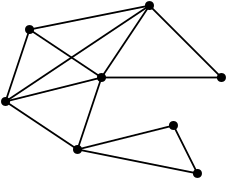
\includegraphics[scale=0.4]{graph}
		\subcaption{}
	\end{minipage}
	\begin{minipage}{0.3\textwidth}
		\centering
		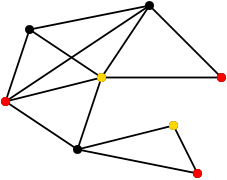
\includegraphics[scale=0.4]{independent_sets}
		\subcaption{}
	\end{minipage}
	\begin{minipage}{0.3\textwidth}
		\centering
		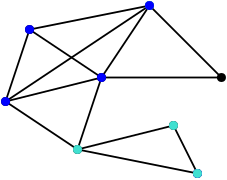
\includegraphics[scale=0.4]{cliques}
		\subcaption{}
	\end{minipage}
	\caption{(a) A connected  graph. (b) Two of its independent sets; one in red (dark) and one yellow (light). The red set constitutes a maximum sized independent set. (c) Two of its cliques; one in blue (dark), one  turquoise (light). The blue  set constitutes a maximum sized clique.}
	\label{fig:is+cliques}
\end{figure}

\begin{lemma}
	\label{lem:vwis}
	\vwis in \NP-complete.
\end{lemma}
\begin{proof}
	First we note that \vwis is in \NP. Indeed, the size of a given set $I$  can be  checked  in  $O(|I|)$ time and it can be verified to be an independent set by checking in time $O(|I|^2)$ whether  any pair  in $|I|$ has an edge  in the  graph. 
	
	We  reduce from \iset.  Let a graph  $G$ and  a parameter $k$ be  given. The intuition behind  the following reduction is the following. We construct a  graph  $H$ with  $V(H)\supset  V(G)$ such that each vertex $v\in  V(G)$ has constant degree  in $H$.  Each independent $I$ in $G$ therefore has volume proportional to $|I|$ in $H$. The trick is then to ensure that each independent set in  $H$ also corresponds to an  independent set  in $I$. Let us proceed with the formalities. 
	
	Let $m=\max_i\deg_G(i)$  be the maximum degree of any vertex in $G$. Construct $H$ as follows. For each vertex $u\in V(G)$,  define  $\alpha(u)=m-\deg_G(u)$ new vertices  $u_1,\dots,u_\alpha$ and take \[V(H)=V(G)\cup \bigcup_{u\in V(G)} \{u_1,\dots,u_\alpha\}.\]  
	We call the vertices which  were originally in $V(G)$ \emph{real},  and the  newly created vertices \emph{fake}. We  add to $E(H)$ the original  edges in $G$ and several sets  of new  edges. First, we add an edge  between  each real  vertex and all its corresponding fake  vertices ($(u,u_i)$ for $i=1,\dots,\alpha(u)$  and all  $u\in V(G)$), and between all fake vertices  corresponding to a single  vertex. Thus,  each  vertex $u$ and  its  fake  vertices $u_1,\dots,u_\alpha$  form a clique. 
	Next, we add an  edge between  every  pair  of fake vertices, i.e., $(u_i,v_j)$ for  all $u,v\in V(G)$  and $i\in[\alpha(u)]$, $j\in[\alpha(v)]$. Formally then,  
	\begin{equation*}
	V(H) = V(G)	\cup\bigcup_{u\in V (G)}\{(u,u_i):i\in[\alpha(u)]\}\cup\bigcup_{u,v\in V(G)}\{(u_i,v_j):i\in[\alpha[u],j\in[\alpha(v)]\}.
	\end{equation*}
	
	We  claim that $G$ has an independent  set of size $k$ iff $H$ has a vertex weighted independent set of size 
	\[mk + \sum_{i\in V(G)} \alpha(i) .\]
	Consider first an independent  set $I\subset V(G)$ in $G$. Take any vertex  $v\in  V(G)\setminus I$ (this set  is non-empty, else $G$ has  no edges), and let $v_i$ be one of its fake vertices. Consider the set $J=I\cup\{v_i\}\subset  V(H)$.  We claim $J$  is an  independent set. Indeed, all added edges in $H$ involve  fake  vertices.  Hence the vertices  in  $I$  still constitute an independent  set in $H$. Moreover, the  only real vertex with  which $v_i$ shares  an edge  is $v$,  which is not in $I$ by assumption. Hence  $J$ is  an independent  set in $H$. Its volume is
	\begin{align*}
	\vol_H(J)  &= \deg_H(u_i)+\sum_{i\in I}\deg_H(i) \\
	&=  \sum_{v\in V(G)} \alpha(v) + \sum_{i\in  I}(\deg_G(i) + \alpha(i)) = \sum_{v\in V(G)}\alpha(v) + m|I|.
	\end{align*}
	Now  consider an independent set $J$ in $H$. Observe that $J$ contains  at most  a single fake vertex (since all  fake vertices are connected). Moreover, if it  has no fake vertices,  we may add a fake vertex of one of the real   vertices which  is not in  $J$. Consequently, without  loss of  generality we may write $J=I\cup\{v_i\}$ where $I\subset V(G)$ are real vertices  and $v_i$ a fake. The edges in $H$ are  a  superset of those in $G$,  hence  $I$ is an independent  set in $G$. The volume of $J$ in  $H$ is computed in the same  way as above. 
	
	We conclude that $G$ has an independent of  size  $k$ iff  $H$ has an  inpedendent  set of  size $mk+\sum_{i\in (V(G)}\alpha(i)$,  which demonstrates that \mwis is \NP-hard. 
\end{proof}


This result allows us to conclude that certain optimizations problems in hyperacute simplices---thus convex polytopes in general---are \NP-hard. 

\begin{lemma}
	Let $\P$ be a convex polytope with vertex set $V$. The optimization problem 
	\begin{alignat*}{2}
	\min_{I\subset V, I\neq\emptyset} & \quad &&  \frac{\norm{\cent(\P_I)}_2^2}{|I|} \\
	\text{s.t.}&  &&  \la \sv_i,\sv_j\ra=0,\; i,j\in I,
	\end{alignat*}
	is \NP-hard. In particular, it is \NP-hard whenever $\P$ is the combinatorial simplex of a graph. 
\end{lemma}
\begin{proof}
	Let $\P=\splx$ be the combinatorial simplex of a graph $G$. Using that $\la \sv_i,\sv_j\ra = w(i,j)$, the condition that $\la \sv_i,\sv_j\ra =0$ for all $i,j\in I$ translates to $(i,j)\in E(G)$ for all $i,j\in I$. Moreover, Equation \eqref{eq:c(S_U)} in Section \ref{sec:S_G} gives us  
	\begin{align*}
	\frac{|I|}{\norm{c(\splx_I)}_2^2} = w_G(\partial I) = \vol(I),
	\end{align*}
	for $I$ an independent set. 
	The above optimization problem can consequently be formulated as 
	\[\max_{I\subset V(G)} \vol_G(I),\quad  \text{s.t.} \quad I \text{ is an independent set}.\]
	which is precisely the \vwis problem. 
	\end{proof}
	
We can play a similar game by using the relationships furnished by the normalized Laplacian as opposed to the combinatorial Laplacian. Doing this removes the normalizing factor of $|I|$ from the optimization problem in the previous result.  

\begin{lemma}
	Let $\P$ be a convex polytope with vertex set $V$. The optimization problem
	\begin{alignat*}{2}
	\min_{I\subset V, I\neq \emptyset} & \quad &&  {\norm{\cent(\P_I)}_2^2} \\
	\text{s.t.}&  &&  \la \sv_i,\sv_j\ra=0,\; i,j\in I,
	\end{alignat*}
	is \NP-hard. In particular, it is hard for those polytopes and simplices with all vertices on the unit sphere. 
\end{lemma}
\begin{proof}
	The proof is similar to the previous lemma. For $\P$ the normalized simplex of a graph $G$, the condition $\la \sv_i,\sv_j\ra=0$ once again implies that $I$ must be an independent set. As before, notice that for such an $I$, if $i\in I$ then $\partial(i) \cap I^c = \partial(i)$ (none of $i$'s neighbours are in $I$). Moreover, for $i,j\in I$, $w(i,j)=0$.  Therefore, Equation \eqref{eq:Lnf(chiU)} yields 
	\begin{align*}
	\Lnf(\bchi_I)=\sum_{i\in I}\frac{1}{w(i)}\sum_{j\in I^c\cap \partial(i)} w(i,j) = \sum_{i\in I}\frac{w(i)}{w(i)} = |I|.
	\end{align*}
	The  length  of the centroid  $\P_I$  is  then 
	\begin{align*}
	\norm{c(\P_I)}_2^2=\frac{1}{|I|^2}\bchi_I^\tp\Svn^\tp\Svn\bchi_I= \frac{1}{|I|^2}\Lnf_G(\bchi_I) =\frac{1}{|I|},
	\end{align*} 
	so the optimization problem can be formulated as 
	\[\max_{I\subset V(G)} |I|,\quad  \text{s.t.} \quad I \text{ is an independent set},\]
	which is the \iset problem. 
\end{proof}

A \emph{clique} in a graph $G$ is a complete subgraph of $G$. The \maxclique problems asks, given  $G$, what is the  largest  $k$ such that $G$ has a clique of size $k$? Its decision version variant, \kclique, has parameters $G$ and $k$, and asks whether $G$ has a clique of size $k$. Karp~\cite{karp1972reducibility} demonstrated that $\kclique\in\NP$ and $\maxclique\in\NP$-hard.  

\begin{lemma}
	Given a polytope in either  \vdesc or \hdesc, consider finding a subset $U$ of the vertices such that none of the vertices in $U$ are orthogonal. The optimization version  of these problem is \NP-hard  while the  decision variant is \NP-complete, even in the case of hyperacute simplices. 
\end{lemma}
\begin{proof}
	The optimization version corresponds to \maxclique while the decision variant corresponds to \kclique via the correspondence.   
\end{proof}



Next we extract a result based on the most (in)famous problem in computational graph theory: Graph isomorphism. An \emph{isomorphism} between two graphs $G_1$ and $G_2$ is a bijection $f:V(G_1)\to V(G_2)$ such that $(u,v)\in E(G_1)$ iff $(f(u),f(v))\in E(G_2)$. We write $G_1\cong G_2$ if $G_1$ is isomorphic to $G_2$. The \graphiso problem asks, given $G_1,G_2$, whether they are isomorphic. 
It's clear that $\graphiso\in\NP$, but whether it is \NP-complete remains an open question~\cite{mckay2014practical}. L{\'a}szl{\'o} Babai recently claims to have solved the problem in  quasipolynomial time~\cite{babai2016graph}; the work is still being verified. 
Accordingly, we call a problem \emph{Graph Isomorphism Hard} if it can be reduced to to \graphiso. 
The more general problem of \emph{subgraph} isomorphism, which asks whether $G_1$ has a subgraph isomorphic to $G_2$, is \NP-complete~\cite{cook1971complexity, karp1972reducibility}. We are interested in the relationship between graph isomorphism and polytope congruence.  

\begin{theorem}
	\label{thm:simplex_congruence}
Deciding whether two hyperacute simplices are congruent is Graph Isomorphism Hard. Moreover, given two hyperacute simplices $\splx_1\in\R^d$ and $\splx_2\in\R^k$, deciding whether there exists $k$-dimensional face of $\splx_1$ congruent to $\splx_2$ is \NP-hard. 
\end{theorem}
\begin{proof}
	Let two graphs $G_1$ and $G_2$ be given. Compute their corresponding inverse simplices $\splx_1^+$ and $\splx_2^+$ (which  takes polynomial time  by  computing  the eigencomposition of both graphs---see Section~\ref{sec:algorithmics_transitions}). 
	We claim that $\splx_1^+\cong\splx_2^+$ iff $G_1\cong G_2$. If $\splx_1^+\cong\splx_2^+$ then because they are both centred at the origin there exists a rotation matrix $\Q$ such that $\Q\Sv_1^+=\Sv_2^+$. Since a rotation matrix does not change the relationship between the inner product of vectors\footnote{A rotation matrix $\Q$ obeys $\Q^\tp\Q=\I$, hence $\la \Q\u,\Q\v\ra = \u^\tp \Q^\tp \Q\v=\la \u,\v\ra$.}, we see that $(\Sv_1^+)^\tp\Sv_1^+$ and $(\Sv_2^+)^\tp\Sv_2^+$ define the same Laplacian. Hence $G_1$ is isomorphic to $G_2$. Conversely, if $G_1\cong G_2$, then there exists a  relabelling of the vertices such that their Laplacian matrices are identical, as are the simplices. This completes  the proof of the first statement. The  follows by a similar reduction, and the fact that $\subgraphiso\in\NP$-complete.
\end{proof}

Kaibel and Schwarz~\cite{kaibel2008complexity} investigated the problem of polytope isomorphism. They define two polytopes as isomorphic if they have the same \emph{face-lattice}---the lattice in which the nodes correspond to subsets of the vertices, and the lattice ordering is by face inclusion. Since congruent simplices share the same face  lattice up to labelling, Theorem \ref{thm:simplex_congruence} implies their result. 


\section{There and Back Again: A Tale of Graphs and Simplices}
\label{sec:algorithmics_transitions}
In this section we investigate the computational aspects of transitioning between the various objects which we've studied thus far. As one should expect given that the mapping between graphs and simplices relies on the  eigenvalues and eigenvectors of graph  Laplacians, the complexity of these transitions is intimately related with the complexity of computing  eigendecompositions. 
As we will see, if we are prepared to compute  eigendecompositions, then we can compute all the objects from one another. 
However, since solving the eigendecomposition is expensive in general (see below), we are mainly interested in circumstances in which a transition can be computed without resorting to this. Unfortunately, it will become clear that the complexity of  computing a Laplacian eigendecomposition is actually a lower bound to computing many of the transitions. 
 
Let $M(n)$ denote the complexity of the eigendecomposition problem. It is known that  $M(n)=\tOmega(n^3 + n\log^2 \log \eps)$ to obtain a relative error\footnote{We note that the relative error is a necessary parameter of any algorithm because eigenvalues may be irrational.} of $2^{-\eps}$, while there exists algorithms which run in time $O(n^3 + n\log^2 \log \eps)$~\cite{pan1999complexity}.  
Let \lapdecomp refer to the problem of computing the eigendecomposition of the Laplacian (either the combinatorial or normalized)of a graph, i.e., computing its eigenvalues and eigenvectors. The complexity of \lapdecomp does not seem to be known  in general, and we thus denote the lower bound by $\Omega(n^\tau)$ for some $\tau$. We will assume, based on the difficulty of general eigendecomposition that $\tau>2$. 


Observe that given $G$, we can compute the combinatorial and nornalized simplices (and their inverses) by first constructing the combinatorial or normalized Laplacian in $O(n^2)$, performing an eigendecomposition in time $O(n^\tau)$, and constructing the vertices of the simplices from the eigenvalues and eigenvectors in time $O(n^2)$. Using our  assumption that $\tau>2$, this takes total time $O(n^\tau)$.  Moreover, starting with a simplex with vertex set $\Sv$, one can compute $\Sv^\tp\Sv$ in the time required for matrix multiplication, which is currently $O(n^{2.3727})$~\cite{williams2012multiplying} and whose lower bound is $\Theta(n^\kappa)$ for some $2\leq \kappa\leq 2.3727$~\cite{stothers2010complexity}. If the simplex is the simplex of a graph then this yields the Laplacian (or its pseudoinverse) in time $O(n^{2.3727})$,  and from here any of its simplices  in time $O(n^\tau)$. Hence, we can transition between the various simplices in time $O(n^{\max\{2.3727,\tau\}})$.  In what follows therefore, we attempt to beat the barrier of $O(n^\tau)$. 

Besides  the question  of transitioning between various objects, we might be interested in the issue of \emph{certification}. That is, verifying whether  a given simplex is one of the combinatorial or normalized simplices of a graph. We will investigate  this question at  the end of this  section. 

\textbf{Nota Bene:} Throughout this section, when referring to the complexity  of generating a graph, we mean the complexity of generating any data structure which describes its connectivity; that is,  lists its  edges (and their weights, if applicable). Formally, the edge weights should be accessible  in $O(1)$ time. The Laplacian matrix,  adjacency matrix, incidence matrix,  etc.,  all suit this  purpose.  Similarly, when discussing the problem of  generating a simplex \emph{from} a graph,  we assume access to such a data structure. We remark that the the normalized Laplacian matrix is \emph{not} such a structure; it  provides no  immediate  access to the  edge weights.

We begin by investigating the relationship between $\splx$ and $\splxn$, when either  $\splx$ or $\splxn$ are given and we are told a priori that they are the simplices of a graph. The results obtained  in this section are summarized in Figure~\ref{fig:mapping_results}. 

\begin{figure}
	\centering
	\renewcommand{\arraystretch}{1.5}	\begin{tabular}{|c|c|c|c|c|c|c|c|c|c|c|}
		\hline 
		\multicolumn{3}{|c|}{} & \multicolumn{4}{c|}{\textsf{V}} & \multicolumn{4}{c|}{\textsf{H}}\\
	\cline{3-11} 
\multicolumn{2}{|r|}{From/To} & $G$ & $\splx_G$ & $\splx_G^+$ & $\splxn_G$ & $\splxn_G^+$ & $\splx_G$ & $\splx_G^+$ & $\splxn_G$ & $\splxn_G^+$ \\
\cline{2-11} 
& $G$ & --- &$\Omega(n^\tau)$ &$\Omega(n^\tau)$ &$\Omega(n^\tau)$ &$\Omega(n^\tau)$ & $\Omega(n^\tau)$ & $\Omega(n^\tau)$ &  & \\
\hline 
\multirow{4}{0.4cm}{\textsf{V}} & $\splx_G$ & $O(n^3)$ & --- & $\Omega(n^\tau)$ & $O(n^2)$ & & $\Omega(n^\tau)$ & $O(1)$ & & \\
\cline{2-11}
& $\splx_G^+$ & & $\Omega(n^\tau)$ & --- & & & $O(1)$ &$\Omega(n^\tau)$ & & \\
\cline{2-11}
& $\splxn_G$ & & ?  / $O(n^2)$ &  & --- & $\Omega(n^\tau)$ & & & &\\
\cline{2-11}
& $\splxn_G^+$ & & & &$\Omega(n^\tau)$ & --- & & & & \\
\hline 
\multirow{4}{0.4cm}{\textsf{H}} & $\splx_G$ & & $\Omega(n^\tau)$ & $O(n^2)$ & & &--- & $\Omega(n^\tau)$& & \\
\cline{2-11}
& $\splx_G^+$ & & $O(n^2)$ & $\Omega(n^\tau)$ & & &$\Omega(n^\tau)$ & --- & & \\
\cline{2-11}
& $\splxn_G$ & & & & &  & & & --- &\\
\cline{2-11}
& $\splxn_G^+$ & & & & & & & & & --- \\
\hline 
	\end{tabular}
	\renewcommand{\arraystretch}{1}
\caption{Summary of results for precise mappings. A slash refers to a difference in runtimes when the graph is available versus when it isn't. The quantity before the slash indicates the runtime \emph{without} the graph, after the slash the runtime \emph{with} the graph. A question mark or empty square indicates that no bounds are yet known. }
\label{fig:mapping_results}
\end{figure}

\paragraph{Between \texorpdfstring{$\splx$}{the combinatorial} and \texorpdfstring{$\splxn$}{normalized simplex}.}
Let us consider the computational complexity of transitioning between $\splx$ and $\splxn$ and vice versa. Let $\phi_{ij}$ (resp., $\phin_{ij}$) be the angle between $\sv_i$ and $\sv_j$ (resp., $\svn_i$ and $\svn_j$). Using the typical formula for the dot product in Euclidean space we have
\begin{equation*}
\cos\phi_{ij} = \frac{\la \sv_i,\sv_j\ra }{\norm{\sv_i}_2\norm{\sv_j}_2} = \frac{\L_G(i,j)}{\sqrt{w(i)w(j)}} = \Ln_G(i,j), \quad\text{and}\quad \cos\phin_{ij} = \frac{\la \svn_i,\svn_j\ra }{\norm{\svn_i}_2\norm{\svn_j}_2} = \Ln_G(i,j),
\end{equation*}
since  $\norm{\svn_i}_2=1$ for all $i$. 
That is, the angles between vertices in $\splx$ in $\splxn$ are the same. Suppose we are given the simplex $\splx$ and told it is the combinatorial simplex of a graph. For each $\sv_i = \Sv(\splx)$, define a new vertex 
\[\bgamma_i = \frac{\sv_i}{\norm{\sv_i}_2}.\]
Is it evident that the angle between $\bgamma_i$ and $\bgamma_j$ is identical to that between $\sv_i$ and $\sv_j$: 
\begin{equation*}
\frac{\la \bgamma_i,\bgamma_j\ra}{\norm{\bgamma_i}_2\norm{\bgamma_j}_2} = \bigg\la \frac{\sv_i}{\norm{\sv_i}_2},\frac{\sv_j}{\norm{\sv_j}_2}\bigg\ra = \cos(\phi_{ij}).
\end{equation*}
 Therefore, the simplex  $\conv(\{\bgam_i\})$ (the $n$ vectors $\{\bgam_i\}$ remain affinely independent) has all of its vertices on the unit sphere and the angle  between each pair of vertices is the  same as in $\splxn$. Thus, this simplex is rotationally congruent  to $\splxn$. This yields the following.

\begin{lemma}
	Given a combinatorial simplex $\splx$, a simplex congruent to $\splxn$ can be computed in time $O(n^2)$. 
\end{lemma}
\begin{proof}
	Given $\splx$, define the vertices $\bgamma_i$ as above. Computing $\norm{\sv_i}_2$ takes time $O(n)$ and must be done for each vertex. 
\end{proof}

Given the relative ease with which we can transition from $\splx$ to $\splxn$, it is somewhat surprising that it is much more difficult to transition from $\splxn$ to  $\splx$, especially if the underlying graph $G$ is not given. The obvious tactic is, given the vertices $\{\svn_i\}$, to define vertices $\svn_i \sqrt{w(i)}$, which, since $\sqrt{w(i)}=\norm{\sv_i}_2$, have the same magnitude as $\sv_i$. As above, the scaling does not affect the angle between the vertices, and thus the simplex with these vertices is congruent to $\splx$. However, it's not clear how to obtain the value $\sqrt{w(i)}$ from $\splxn$. Using that $\la \svn_i,\svn_j\ra =(w(i)w(j))^{-1/2}$ we can write 
\[w(i)^{1/2} = -\sum_{j\neq i}w(j)^{-1/2} \bigg/ \sum_{j\neq i}\la \svn_i,\svn_j\ra,\]
which yields a non-linear system of equations. 

Of course, if we are given the graph then we have access to $\sqrt{w(i)}$ and can compute $\svn_i w(i)^{1/2}$ in time $O(n)$. The following result is then immediate. 

\begin{lemma}
	Given a graph $G=(V,E,w)$ and its normalized simplex $\splxn_G$, a simplex congruent to  the combinatorial simplex $\splx_G$ can be computed in $O(n^2)$ time. 
\end{lemma}

%\note{Think about possible lower bounds on computing $\splx$ from $\splxn$ when no graph is given. Doing so would imply knowledge of $\sqrt{\w}$ (taking ratio of lengths of vertices). What does this imply? Does knowledge of $\w$ give us some knowledge of the graph structure from which we can extract a lower bound? }



\paragraph{\texorpdfstring{$\splx$}{The combinatorial} and \texorpdfstring{$\splx^+$}{normalized simplex}.}

Let us suppose that we can generate $\splx^+$ from $\splx$ (or vice versa) in time $O(g(n))$. Note that for $i<n$, 
\begin{equation}
\label{eq:decomp_from_vertices}
\lambda_i = \frac{\lambda_i^{1/2} \vp_j(i)}{\lambda_i^{-1/2}\vp_j(i)} = \frac{\sv_i(j)}{\sv_i^+(j)}, \quad \text{and} \quad \vp_i(j) = \frac{\sv_j(i)}{\lambda_i^{1/2}},
\end{equation}
hence knowledge of $\{\sv_i\}$ and $\{\sv_i^+\}$ yields knowledge of the eigendecomposition of the underlying graph $G$ in $O(n^2)$ time ($O(n)$ to determine all the  eigenvalues and $O(n^2)$ to determine the eigenvectors). The same argument holds \emph{mutatis mutandis} for the normalized Laplacian. 

\begin{lemma}
	\label{lem:S_to_S^+_vdesc}
	If a \vdesc of $\splx^+$  (resp., $\splxn^+$) can be generated from a \vdesc of $\splx$ (resp., $\splxn$) or vice versa in time $O(g(n))$, then \lapdecomp can be solved in time $O(g(n) + n^2)$ for arbitrary weighted graphs. Consequently $g(n) = \Omega(n^\tau)$.  
\end{lemma}

An alternate way of seeing that constructing the inverse simplex from its dual is computationally challenging is to recall from Section \ref{sec:S_G} that $\splx_\ic$ is contained in the hyperplane $\{\x\in\R^{n-1}:\la \x,\sv_i^+\ra = -1/n\}$ (Lemma \ref{lem:SUsubset})
 and that $\sv_i^+$ is perpendicular to $\splx_\ic$ (Lemma \ref{lem:S_G_basic_properties}). Hence, computing the inverse simplex would imply that we had computed normal vectors to $n$ hyperplanes, the typical procedure which typically involves computing an $n\times n$ determinant and requires  $O(n^3)$ time. 
 
 We now consider transitioning between different descriptions of $\splx$ and $\splx^+$. Let us recall that the \hdesc of $\splx$ and $\splx^+$ yield immediate insight into the vertices of its inverse as $\splx=\cap_i \{\x:\la \x,\sv_i^+\ra \geq -1/n\}$ and $\splx^+=\cap_i\{\x:\la\x,\sv_i\ra \geq -1/n\}$ (Equations \eqref{eq:splx_bigcapH_i} and \eqref{eq:splx^+_bigcapH_i}). Consequently, given a \hdesc of one of these simplices, the vertices of its inverse are recoverable in quadratic time. This observation will be used several times and is  worth encoding. 
 
 \begin{observation}
 	\label{obs:HtoV}
 	Given  an  \hdesc of $\splx$ (resp., $\splx^+$)  the vertices of $\splx^+$ (resp., $\splx$) are obtainable in quadratic time.
 \end{observation}
\begin{proof}
	An \hdesc of $\splx$  involves parameters  $\u_1,\dots,\u_n$ and $\beta_1,\dots,\beta_n$ such that $\splx=\cap_i \{\x:\la \x,\v_i\ra \geq  \beta_i\}=\{\x:\la \x,-\u_i/(n\beta_i )\geq -\frac{1}{n}\}$. Using  Equation~\eqref{eq:S_alt_desc} (also written above) shows  that $\sv_i^+=-\u_i/(n\beta_i)$.  Computing this  for all $i$ requires  times  $O(n^2)$ (we need  to obtain each coordinate).  
\end{proof}
 
 This immediately  leads to the following bound on computing an \hdesc from a \vdesc. 
 
 \begin{lemma}
 	\label{lem:S_vdesc_to_hdesc}
	 Suppose that in time $t(n)$ we can compute an \hdesc of $\splx$ (resp., $\splx^+$) given its \vdesc. Then a \vdesc of $\splx^+$ (resp., $\splx$) is recoverable in time $t(n) + O(n^2)$, implying by Lemma \ref{lem:S_to_S^+_vdesc} that $t(n) = \Omega(n^\tau)$. 
 \end{lemma}

We also note that a consequence of the relationship between the vertices of $\splx$ and the \hdesc of $\splx^+$ is that given the \vdesc of $\splx$ or $\splx^+$, we have immediate---that is,  $O(1)$ time---access to the \hdesc of its inverse. 

A similar result holds for transitioning between the \hdesc of the combinatorial simplices. The argument runs as usual: Given an \hdesc of $\splx$, suppose we can generate an \hdesc of $\splx^+$ in time $t(n)$. We can obtain the vertices $\{\sv_i^+\}$ from the \hdesc of $\splx$, and the vertices $\{\sv_i\}$ from the \hdesc of $\splx^+$. Using these, we can then obtain the eigendecomposition of $G$ in time $O(n^2)$. That is, we can solve \lapdecomp in time $t(n) + O(n^2)$ yielding that $t(n) = \Omega(n^\tau)$. 

\begin{lemma}
	\label{lem:hdesc_to_hdesc}
	Generating an \hdesc of $\splx_G$ given an \hdesc of $\splx_G^+$, and vice versa, requires time $\Omega(n^\tau)$. 
\end{lemma}


\paragraph{Between \texorpdfstring{$G$}{the graph} and \texorpdfstring{$\splx$ or $\splxn$}{its simplices}.}
Similar lower  bounds  hold in this case. First, suppose that we obtain a \vdesc of $\splx_G$ from $G$. Notice  that \[\sum_{i=1}^{n-1}   \sv_i(j)^2 = \lambda_j \sum_{i=1}^{n-1} \vp_j(i)^2 = \lambda_j\bigg(1-\frac{1}{n}\bigg),\]
so 
\[\lambda_j = \frac{\sum_{i=1}^{n-1}\sv_i(j)^2}{1-1/n},\]
which can be computed  in $O(n)$  time. Then, as per Equation~\eqref{eq:decomp_from_vertices}, knowledge of the eigenvalues furnishes knowledge  of the eigenvectors in $O(n^2)$ time. This implies that obtaining such a \vdesc requires $\Omega(n^\tau)$ time. Running almost identical arguments for $\splx^+$, $\splxn$, or $\splxn^+$ gives the  following. 

\begin{lemma}
	\label{lem:G_to_S_and_Sn}
	If the \vdesc of the combinatorial simplex, the normalized simplex, or their  inverses can be generated from a graph $G$ in $O(g(n))$ time, then \lapdecomp can be solved in time $O(g(n) + n^2)$ for arbitrary weighted graphs. Consequently $g(n) = \Omega(n^\tau)$. 
\end{lemma}

The prospects are  equally  as bleak for generating an \hdesc from $G$. The argument is  similar. 

\begin{lemma}
	Given a graph $G$ suppose an \hdesc of $\splx$ (resp., $\splx^+$) can be generated in time $g(n)$. Then a \vdesc of $\splx^+$ (resp., $\splx$ can be obtained in time $O(g(n) + n^2)$ by Observation~\ref{obs:HtoV}. Consequently, by Lemma \ref{lem:G_to_S_and_Sn}, $g(n)=\Omega(n^\tau)$. 
\end{lemma}

\todo 
Next we examine generating the graph  from various simplices. We first require the following result. It is intuitively  obvious but we err on  the side of verifying it. 

\begin{observation}
	Any algorithm which  determines whether two vertices in  $\R^n$ are  orthogonal requires  $\Omega(n)$ time. 
\end{observation}
\begin{proof}
	Let $\mA$ be a purported sublinear time algorithm which performs this  task. Let $\x,\y\in\R^n$ be  two inputs  to  $\mA$. Assume they  both  contain no zero entries ($\mA$ claims to work  for  all vectors). Since  $\mA$ is sublinear, there exists some $i\in[n]$ such that $\mA $ does not  examine $x(i)$. Therefore,  we may  vary $x(i)$ without changing  $\mA$'s  output. If $\mA$ output ``yes'', meaning that it believes $\x$ and $\y$ to be orthogonal, put 
	\[x(i) = \frac{1-\sum_{j\neq i}x(j)y(j)}{y(i)}.\]
	Then  $\la \x,\y\ra =1$, so they are are not orthogonal. Similarly,  if $\mA$ output ``no'', then put 
	\[x(i) = -\frac{\sum_{j\neq i}x(j)y(j)}{y(j)},\]
	so  that $\la\x,\y\ra=0$. Therefore, $\mA$ cannot  be  correct on all inputs.  
\end{proof}

This allows us to give the precise complexity required for  generating the graph from its  combinatorial  simplex.  

\begin{lemma}
	Given a  \vdesc  of  $\splx_G$,  computing the underlying graph  $G$ requires $\Omega(n^3)$ time. It can be done in time $O(n^3)$. 
\end{lemma}
\begin{proof}
	We begin with the second statement. Given $\{\sv_i\}$ we can compute the weight between vertex $i$ and  $j$ as  $\la \sv_i,\sv_j\ra=-w(i,j)$ which  requires linear time. Performing the computation for all pairs and thus obtaining all the edge information takes $O(n^3)$  time. 
	The lower  bound 
\end{proof}




\paragraph{Between different descriptions of the simplices.}
Here we investigate  the interplay between the various different descriptions of the simplices. The  arguments are largely similar  to those in the section on  transitioning between  $\splx$ and $\splx^+$. 

The following is an immediate consequence of Lemma \ref{lem:hdesc_dual} and Observation~\ref{obs:HtoV}. It applies to all simplices.  

\begin{corollary}
	\label{cor:hdesc_S_to_S+}
	If $\ssplx$ is a centred simplex in \hdesc, we can obtain a \vdesc of $\ssplx^\du$ in quadratic time. In particular, given  an \hdesc of the combinatorial simplex $\splx_G$ (resp., inverse combinatorial  simplex $\splx_G^+$)  of a graph $G$, a \vdesc of $\splx_G^+$ (resp., $\splx_G$)  is obtainable in quadratic time. 
\end{corollary}

Due to the fact that $\splxn_G^+$ is not the dual of $\splxn_G$,  it is difficult to  see how to  obtain a similar result  for the normalized simplex. 

\begin{lemma}
	\label{lem:hdesc_to_vdesc}
	Generating a \vdesc of the simplex $\splx$ given its \hdesc requires time $\Omega(n^\tau)$ for any $\splx\in\{\splx_G,\splx_G^+\}$. 
\end{lemma}
\begin{proof}
	Consider $\splx_G$; the argument is similar for $\splx_G^+$. Suppose obtaining the \vdesc takes time $t(n)$. Due to the properties of the hyperplane representations, this yields access to both sets of vertices ($\{\sv_i\}$ and $\{\sv_i^+\}$) in time $t(n)+O(n^2)$ (Observation~\ref{obs:HtoV}). Using Equation~\eqref{eq:decomp_from_vertices}, this implies that we can obtain the eigenvalues and eigenvectors of $G$ in time $O(n^2)$, i.e., we can solve \lapdecomp in time $t(n)+O(n^2)$. Hence $t(n)=\Omega(n^\tau)$. 
\end{proof}


\paragraph{Verification.}
We  now turn  to discussing the complexity of  verifying whether  a given simplex is the simplex of graph. 
In time $O(n^{2.3727})$ we can compute $\Sv^\tp\Sv$. We can check whether this is equal to $\L_G$ for some $G$ by verifying whether (i) $\Sv^\tp\Sv\one=\zero$, (ii) $(\Sv^\tp\Sv)(i,i)>0$ for all $i$ and (iii) $(\Sv^\tp\Sv)(i,j)\leq 0$ for all $i\neq j$. These three steps require time $O(n^3)$. We can check whether $\Sv^\tp\Sv$ is equal to $\Ln_G$ for some $G$ by first ensuring, similarly to above, that (iii) holds and that $(\Sv^\tp\Sv)(i,i)=1$ for all $i$. Then we compute the kernel  of $\Sv^\tp\Sv$ in cubic time by means of Gaussian elimination~\cite{kailath1999fast} to obtain a vector $\v$ equal to $\sqrt{\w_G}$ (if indeed $\Sv^\tp\Sv=\Ln_G$) up to scaling. To determine whether $\v$ does represent valid weightings of the vertices, we check whether $(\Sv^\tp\Sv)(i,j)\v(j)$ is constant for all $i$. In  this case $\Sv^\tp\Sv$ is equal to the normalized Laplacian of some graph. This can also be done in cubic time. We  therefore see that we can  verify whether a given simplex is the combinatorial or  normalized simplex of a graph in  cubic time. It's not clear whether it can be done faster, however. 

Finally, we note that in cubic time we can check whether all the angles $\theta_{ij}$ between the faces $\ssplx_\ic$ and $\ssplx_\jc$ are non-obtuse, in which case $\ssplx$ is the inverse simplex of some graph. 


\section{Approximations} 
\label{sec:algorithmics_approximations}
Here we are concerned  with  approximations of various sorts. We begin  with an eye towards the problem of  dimensionality. Specifically, Theorem ~\ref{thm:graph-simplex} yields simplices of dimension $n-1$ for a graph on $n$ vertices. In  many application areas, graphs may have thousands  to  millions of vertices. Working in a Euclidean space  of  this  size can be unwieldy. Our first two  sections,  therefore, attempt dimensionality reduction. The first  considers the problem of reducing the dimensionality of the simplex itself. The second considers low rank approximations of  the Laplacian which are  shown to yield polytopes on  $n$ vertices. We see that, depending on the rank of the  approximation and the eigenvalues of the Laplacian, certain properties of this polytope approximate  those of the simplex. As we will see, this provides some  theoretical justification for  the  recent work of Torres \etal~\cite{torres2019geometric}. 

\subsection{Dimensionality  Reduction: \texorpdfstring{$\splx^+$}{the inverse simplex}}
\label{sec:algorithmics_JL}
Assume we are given one of the simplices of a  graph.  
The idea is to  map each vertex to a  point in $\R^d$, for $d\ll n$, while maintaining the general form of the simplex. By this we mean that we'd like the distance between the new  points  to remain approximately  as they  were. If possible, we'd also  like the new, lower  dimensional  object (note that it won't  be  a simplex because there will  be  $n$ points in $ \R^d$) to retain some of the properties which  relate it  to the underlying graph. In  particular, we'd like the gram matrix  of the new  points to  approximate the gram  matrix of the original  set  of points. As it turns out,  a  mapping meeting both  of these criteria exists and is computable  in polynomial time. It will   rely on the Johnson-Lindenstrauss  (JL) Lemma~\cite{johnson1984extensions,dasgupta2003elementary}. 

\begin{theorem}[Johnson-Lindenstrauss]
	Let $\X\subset \R^k$ be a set of $n$ points, for some $k\in\N$. For any $\eps>0$ and $d\geq 8\log(n)\eps^{-2}$ there exists a map $g_\eps:\R^k\to\R^d$ such that 
	\begin{equation*}
	(1-\eps)\norm{\u-\v}_2^2 \leq \norm{g_\eps(\u) - g_\eps(\v)}_2^2 \leq (1+\eps)\norm{\u-\v}_2^2,
	\end{equation*}
	for all $\u,\v\in \X$. 
\end{theorem}

%Thus $\norm{\sv_i^+-\o}_2^2 = \L_G^+(i,i)$ for all $i$. Note that we can compute this in linear time since 
%\[\norm{\sv_i^+-\o}_2^2 = \norm{\sv_i^+}_2^2 = \frac{1}{W(\partial(\{i\}))}=\frac{1}{w(i)}.\]


Now, let us suppose we have the vertices $\{\sv_i^+\}$ of the inverse simplex (the same argument could be run  with any of the simplices). Let $\X = \{\sv_i^+\}\cup\{\zero\}$. Apply the JL Lemma to $\X$ to  obtain $n+1$ points in $\R^d$, for $d=O(\log(n)/\eps^2)$. Let $f$ be the mapping, e.g., $\sv_i^+$ is sent to $f(\sv_i^+)$. By JL, have 
\[(1-\eps)\norm{\x-\y}_2^2\leq  \norm{f(\x) -f(\y)}_2^2\leq (1+\eps)\norm{\x-\y}_2^2, \]
for all $\x,\y\in \{\sv_1^+,\dots,\sv_n^+,\zero\}$. 
Apply a linear transformation to the points so that $f(\zero)$ coincides with the origin $\zero\in\R^d$. Note that this does not affect the distances between the points themselves, and does not damage the approximation. Update $f$ to reflect this transformation. 
For all $i,j$, let $\eps_{i,j}$ denote the true error of the mapping, i.e., 
\[\norm{f(\sv_i^+)-f(\sv_j^+)}_2^2 = (1+\eps_{i,j})\norm{\sv_i^+-\sv_j^+}_2^2,\]
where $|\eps_{i,j}|\leq \eps$. Define $\eps_{i,\zero}$ similarly. 
Then, 
\[\norm{f(\sv_i^+)}_2^2 = \norm{f(\sv_i^+)-f(\zero)}_2^2 = (1+\eps_{i,\o})\norm{\sv_i^+}_2^2 = (1+\eps_{i,\o})\L_G^+(i,i),\]
hence, 
\begin{align*}
\norm{f(\sv_i^+)-f(\sv_j^+)}_2^2 &= \la f(\sv_i^+)-f(\sv_j^+),f(\sv_i^+)-f(\sv_j+)\ra \\
&= \norm{f(\sv_i^+)}_2^2 + \norm{f(\sv_j^+)}_2^2 - 2\la f(\sv_i^+),f(\sv_j^+)\ra,  
\end{align*}
implying that 
\begin{align*}
\la f(\sv_i^+),f(\sv_j^+) \ra &= -\frac{1}{2} \bigg((1+\eps_{i,j})\norm{\sv_i^+-\sv_j^+}_2^2 - (1+\eps_{i,\o})\L_G^+(i,i) - (1+\eps_{j,\o})\L_G^+(j,j)\bigg) \\
&= -\frac{1}{2}((1+\eps_{i,j})r(i,j) - (1+\eps_{i,\o})\L_G^+(i,i) - (1+\eps_{j,\o})\L_G^+(j,j)) \\
&= -\frac{1}{2}((1+\eps_{i,j})(\L_G^+(i,i) - \L_G^+(j,j) - 2\L_G^+(i,j)) \\
&\hspace{2cm}- (1+\eps_{i,\o})\L_G^+(i,i) - (1+\eps_{j,\o})\L_G^+(j,j))\\
&= (1+\eps_{i,j})\L_G^+(i,j) + \varepsilon(i,j),
\end{align*}
where 
\[\varepsilon(i,j)\equiv \frac{1}{2}(\eps_{i,\o}-\eps_{i,j})\L_G^+(i,i) + (\eps_{j,\o}-\eps_{i,j})\L_G^+(i,j),\]
is an error term dictated by $\eps_{i,j}, \eps_{i,\o}$ and $\eps_{j,\o}$. Setting $M= \max_i \L_G^+(i,i)$ 
we can bound the error term via repeated applications of the triangle inequality: 
\begin{align*}
|\varepsilon(i,j)|& \leq \frac{1}{2}\bigg(|(\eps_{i,\o}-\eps_{i,j})\L_G^+(i,i)| + |(\eps_{j,\o}-\eps_{i,j})\L_G^+(i,j|\bigg) \\
& \leq \frac{1}{2}\bigg([|\eps_{i,j}|+|\eps_{i,\o}|]\L_G^+(i,i) + [|\eps_{i,j}|+|\eps_{j,\o}|]\L_G^+(j,j)\bigg) \\
&\leq \frac{1}{2} ( 2\eps\L_G^+(i,i) + 2\eps\L_G^+(j,j) ) \leq 2\eps M,
\end{align*}
since $|\eps_{i,j}|, |\eps_{i,\o}|,|\eps_{j,\o}|\leq |\eps|$. Setting $f(\Sv^+) = (f(\sv_1^+),\dots,f(\sv_n^+))\in \R^{d\times n}$, this approximation implies that 
\begin{equation*}
\L_G^+ - O(\eps M)\I \leq f(\Sv^+)^\tp f(\Sv^+) \leq \L_G^+ + O(\eps M)\I. 
\end{equation*}
In other words, we can approximately recover the Gram matrix $\L_G^+=\Sv^+\Sv^+$ using the lower dimensional matrix $f(\Sv^+)$. 

The JL mapping also maintains other approximate information of the graph.  For  example,  it is well-known that the effective resistance between two vertices is related to the probability that this edge  is in a random  spanning  tree as 
\begin{equation*}
	\effr(i,j) = \frac{1}{w(i,j)} \Pr_{T\sim \mu}[(i,j)\in T],
\end{equation*}
where $\mu$ is the uniform distribution over all spanning trees~\cite{burton1993local}. Hence, 
\begin{equation*}
\norm{f(\sv_i^+)-f(\sv_j^+)}_2^2 \in \frac{1}{w(i,j)}\bigg[(1-\eps),(1+\eps)\bigg]\Pr_{T\sim \mu}[(i,j)\in T].
\end{equation*}
	

\subsection{Dimensionality Reduction: \texorpdfstring{$\L_G$}{the Laplacian}}
\label{sec:algorithmics_low_rank}
In Section  \ref{sec:algorithmics_JL}, we asked how to reduce the  dimension of the  simplex  while (approximately) maintaining several of its  properties. However,  we might instead  reduce the dimensionality of the  Laplacian. This section explores this prospect. 


Let us suppose the we have obtained a low rank---$k$, say---approximation of $\L_G$, written $\L_k$. We might then ask several questions: 
\begin{enumerate}
	\item Is $\L_k$ still a gram matrix? That is, can $\L_k$ be written $\tSv^\tp\tSv$ where $\tSv$ is the vertex matrix of some set of points, $P=\{\p_1,\dots,\p_\ell\}$? If so, what is the relationship between $\Sv$ and $\tSv$, where $\Sv=\Sv(\splx_G)$ is the usual vertex matrix of the combinatorial simplex of $G$? If $\L_k$ has rank $k$ then $P$ spans a subspace of dimension $k$ and $\conv(P)$ forms a polytope in that space. What is the relationship between the geometry of $\conv(P)$ and $\splx_G$?
	\item Is $\L_k$ useful in helping estimate properties of the simplex $\splx_G$? For example, if one could bound the difference in the quadratic products of $\L_G$ and $\L_k$, this would imply (via the results in Section \ref{sec:S_G}) that we could estimate many of the properties of $\splx_G$. 
\end{enumerate}

Of course, we have chosen to work with $\L_G$ and $\splx_G$ for convenience; we could have asked the same questions of $\Ln_G$ and $\splxn_G$. 

Let us  consider the natural rank-$k$ approximation to $\L_G$: 
\begin{equation*}
\L_k\equiv \sum_{i=1}^k \lambda_k\vp_k\vp_k^\tp,
\end{equation*}
where we recall that  we've ordered  the eigenvalues  as $\lambda_1\geq \lambda_2\geq \dots\lambda_{n-1}>\lambda_n=0$. 
Clearly $\L_k$ has rank $k$.  It is, moreover, a symmetric PSD matrix.  Section~\ref{sec:correspondence_polyhedra_matrices} thus yields the polytope $\P_k\equiv \P_{\L_k}$ associated  with $\L_k$. More  explicitly, if 
$\Eval_k=\diag(\lambda_1,\dots,\lambda_n)$ is the diagonal  matrix containing the first $k$  eigenvalues (meaning those  associated  with  $\lambda_1,\dots,\lambda_k$) and $\Eig_k = (\vp_1\;\dots;\vp_k)$, then $\L_k$ is the Gram matrix of the vertices described be the matrix $\Sv_k = \Eval_k^{1/2}\Eig_k^\tp=(\sv_1^\k,\dots,\sv_n^\k)$ where $\sv_i^\k=(\vp_1(i)\lambda_1^{1/2},\dots,\vp_k(i)\lambda_k^{1/2})$. Let us emphasize that we  are using  the subscript $(k)$ to signify that these vertices are  those belonging to  $\P_k$. 

To  summarize, the rank $k$ approximation to $\L_G$, $\L_k$  yields an  $n$-vertex polytope  $\P_k\subset\R^k$. Naturally, one would hope that $\P_k$    ``approximates'' various features of $\splx_G$, as it is precisely $\splx_G$ projected  onto a particular $k$-dimensional subspace. The next few results  demonstrate that this is true under certain  assumptions placed on the distribution of the eigenvalues. 

The first property worth noticing is that $\P_k$ remains  centred at the  origin. Indeed,  $\cent(\P_k) = \frac{1}{n}\Sv_k\one = \frac{1}{n}\Eval_k^{1/2}\Eig_k^\tp\one=\zero_k$.  Next, we might wonder  whether the lengths of the  centroids to different faces  are similar in $\splx_G$ and $\P_k$. Fix  $U\subset [n]$ and compute 

\begin{align*}
\bigg|\norm{\cent(\splx_G[U])}_2^2 - \norm{\cent(\P_k[U])}_2^2\bigg| &= \frac{1}{|U|^2}\bigg| \bchi_U^\tp \Sv^\tp\Sv\bchi_U - \bchi_U^\tp \Sv_k^\tp\Sv_k\bchi_U \bigg| \\
&= \frac{1}{|U|^2} \bigg|\bchi_U^\tp (\L_G-\L_k)\bchi_U\bigg| \\
&=  \frac{1}{|U|^2} \bigg|\bchi_U^\tp \bigg( \sum_{i\in[n-1]}\lambda_i\vp_i\vp_i^\tp - \sum_{i\in[k]}\lambda_i\vp_i\vp_i^\tp\bigg)\bchi_U\bigg|\\
&\leq  \frac{1}{|U|^2} \sum_{i=k+1}^{n-1}|\lambda_i \bchi_U^\tp \vp_i\vp^\tp\bchi_U |\\
&=   \frac{1}{|U|^2} \sum_{i=k+1}^{n-1}\la \bchi_U,\vp_i\ra^2,
\end{align*}
where, by Cauchy-Schwarz, $\la \bchi_U,\vp_i\ra^2 \leq \norm{\bchi_U}_2^2 \norm{\vp_i}_2^2 = |U|^2$, 
hence  
\begin{align}
\bigg|\norm{\cent(\splx_G[U])}_2^2 - \norm{\cent(\P_k[U])}_2^2\bigg| &\leq \sum_{i=k+1}^{n-1}  \lambda_i  \leq \lambda_{k+1} (n-(k+1)). \label{eq:|cS-cP|}
\end{align}
Thus, if $\lambda_k$ is sufficiently small as a function  of $n$ and $k$, the lengths of the centroids are approximately equal. We summarize with  the following Lemma. 

\begin{lemma}
	If $\lambda_{k+1} = o((n-k)^{-1})$, then  $ \bigg|\norm{\cent(\splx_G[U])}_2^2 - \norm{\cent(\P_k[U])}_2^2\bigg| = o(1)$. 
\end{lemma}
\begin{proof}
	Assume $\lambda_k = o((n-k)^{-1})$ and apply Equation~\eqref{eq:|cS-cP|}. 
\end{proof}

\begin{remark}
	The  above result should seem intuitively plausible.  How  well $\L_k$ approximates $\L_G$ relies precisely on the size of $\lambda_k$. We should  thus expect  the same to be  true  of $\P_k$ and  $\splx_G$. 
\end{remark}

Next, we  investigate the relative distances between  the vertex vectors. The difference  in distances  between the vectors of $\splx_G$ and $\P_k$ is 

\begin{align*}
\bigg| \norm{\sv_i-\sv_j}_2^2 - \norm{\sv_i^\k-\sv_j^\k}_2^2  \bigg| &= \left| \sum_{\ell\in[n-1]} (\sv_i(\ell)-\sv_j(\ell))^2  - \sum_{\ell\in[k]}(\sv_i(\ell) - \sv_j(\ell))^2 \right|\\ 
&= \left| \sum_{\ell\in[n-1]} \lambda_\ell(\vp_\ell(i)-\vp_\ell(j))^2  - \sum_{\ell\in[k]}\lambda_\ell(\vp_\ell(i) - \vp_\ell(j))^2 \right|\\ 
&=\left| \sum_{\ell=k+1}^{n-1} \lambda_\ell(\vp_\ell(i)-\vp_\ell(j))^2 \right|\\ 
&\leq \lambda_{k+1} \sum_{\ell=k+1}^{n-1} |\vp_\ell(i)-\vp_\ell(j)|^2.
\end{align*}
The  goal is  thus to bound the final summation in  terms of some function of $n$ or $k$, so that we may provide sufficient conditions on $\lambda_{k+1}$ in order for $\norm{\sv_i^\k-\sv_j^\k}_2^2$ to approximate $\norm{\sv_i-\sv_j}_2^2$. We proceed as follows. 
\begin{align*}
\sum_{\ell=k+1}^{n-1} |\vp_\ell(i)-\vp_\ell(j)|^2 &= \bigg|\sum_{\ell=k+1}^{n-1} |\vp_\ell(i)-\vp_\ell(j)|^2\bigg| \\
&= \bigg|\sum_{\ell={k+1}}^{n-1} \vp_\ell(i)^2 + \vp_\ell(j)^2 - 2\vp_\ell(i)\vp_\ell(j) \bigg|\\
&\leq \sum_{\ell=k+1}^{n-1} \vp_\ell(i)^2 + \sum_{\ell=k+1}^{n-1} \vp_\ell(j)^2 + 2\bigg|\sum_{\ell=k+1}^{n-1} \vp_\ell(i)\vp_\ell(j)\bigg| \\
&\leq \sum_{\ell=k+1}^{n-1} \vp_\ell(i)^2 + \sum_{\ell=k+1}^{n-1} \vp_\ell(j)^2 + 2\bigg(\sum_{\ell=k+1}^{n-1}\vp_\ell(i)^2\sum_{m=k+1}^{n-1}\vp_m(j)^2\bigg) ^{1/2} \\
&\leq \sum_{\ell\in[n]} \vp_\ell(i)^2 + \sum_{\ell\in[n]}^{n-1} \vp_\ell(j)^2 + 2\bigg(\sum_{\ell\in[n]}^{n-1}\vp_\ell(i)^2\sum_{m=k+1}^{n-1}\vp_m(j)^2\bigg) ^{1/2}. 
\end{align*} 
Now,  recall that due to double orthogonality of the eigenvector matrix we  have $\sum_{\ell=1}^n \vp_\ell(i)\vp_\ell(j) = \delta_{ij}$.  The above quantity is therefore  equal to 6. Consequently, combining the previous few equations yields 
\begin{equation*}
\bigg| \norm{\sv_i-\sv_j}_2^2 - \norm{\sv_i^\k-\sv_j^\k}_2^2\leq 6\lambda_{k+1}=O(\lambda_{k+1}). 
\end{equation*}

\begin{lemma}
	If $\lambda_{k+1}=o(1)$ then $\bigg| \norm{\sv_i-\sv_j}_2^2 - \norm{\sv_i^\k-\sv_j^\k}_2^2= o(1)$. 
\end{lemma}

Summarizing, we see  that under assumptions on the sizes of the eigenvalues (which relates  directly to  how good of an approximation $\L_k$ is to $\L_G$), the features of the  polytope $\P_k$  will  approximate  those of $\splx_G$. As we stated previously, this could help explain in part the success of the experiments run by Torres \etal~\cite{torres2019geometric}.  In their work, they assume they are given  $\P_k$ and  attempt to reconstruct certain  graph  features,  most notably its connectivity.  Since  the connectivity of  a  graph  is related to  the centroids of $\splx_G$ (Section~\ref{sec:S_G}), if $k$ is sufficiently small then  the centroids $\P_k$ will approximately  recover the edge relations. 




\subsection{Distance Matrix of \texorpdfstring{$\splx_G^+$}{the inverse combinatorial simplex}}
\label{sec:algorithmics_distance_matrix}
We end with  a brief section which demonstrates that we can leverage several results from the literature on Laplacian optimization to approximate the  distance matrix  of $\splx_G^+$. 
An elegant result of Spielman and Srivastava~\cite{spielman2011graph} allows us to  build a matrix which approximately  represents the effective resistances.  


\begin{theorem}[\cite{spielman2011graph}]
	\label{thm:er_approximation}
	For any $\eps>0$ and graph $G=(V,E,w)$, there exists an algorithm which computes a matrix $\widetilde{\Reff}\in\R^{O(\log(n)\eps^{-2})\times n}$ such that 
	\begin{equation*}
	(1-\eps)r(i,j) \leq \norm{\widetilde{\Reff}(\bchi_i-\bchi_j)}_2^2 \leq (1+\eps) r(i,j).
	\end{equation*}
	The algorithm runs in time $\widetilde{O}( |E|\log (r)/\eps^2)$, where 
	\[r=\frac{\max_{i,j}w(i,j)}{\min_{i,j}w(i,j)}.\]
\end{theorem}


Therefore, given a graph $G=(V,E,w)$, we use the algorithm of Theorem \ref{thm:er_approximation} to compute all the approximate distances $\norm{\sv_i^+-\sv_j^+}_2^2=\effr(i,j)$ in time \[\widetilde{O}(|E|\log (r)/\eps^2)+O(|E| \log(n)/\eps^2)=\widetilde{O}(|E|/\eps^2),\]
assuming $r=O(1)$. Note that we can compute a single effective resistance in time $O(\log n/\eps^2)$, since it involves simply computing the $\ell_2$ norm the vector $\widetilde{\Reff}(\bchi_i-\bchi_j)$ which is simply the difference of two columns of $\widetilde{\Reff}$. 

Ideally, after computing  $\widetilde{\Reff}$, we'd like to compute vertices which (approximately) obey the  distances represented by $\widetilde{\Reff}$ (note  that $\widetilde{\Reff}$ may not be a valid distance matrix since it  is only an approximation). The usual approach to generating points from a (true) distance matrix $\D$ is \emph{Multidimensional Scaling (MDS)}~\cite{kruskal1978multidimensional}. Typically, practitioners are interested  in  generating points which approximately  obey the pairwise distance in  $\D$, but  lie in a lower dimensional space. 
While  this sounds promising, MDS relies on the the eigendecomposition of the distance matrix which requires cubic time. Of  course, this is too slow for our  purposes:  If we allow cubic time, then we can simply perform an  eigendecomposition of $\L_G$ and recover the vertices of $\splx_G^+$ exactly. Moreover, it's unclear whether MDS works when  the given distances are  only approximate. 


We therefore  leave the reader with  the  following open problem:  

\textbf{Problem:} Given an approximate Euclidean distance matrix $\tD$ and a parameter  $\eps>0$, can a set of vertices be computed which  obey  the distances given by $\tD$ within an additive factor of $\eps$  in sub-cubic time? 










